\section{Software \& Code Implementation}

This section describes the software developed for the Bako OBD ISS platform, covering the embedded firmware running on the ESP32 microcontroller, the battery management decoding logic, the cloud publishing pipeline, and the validation strategy used to verify correct behavior at each layer.

% ─────────────────────────────────────────────────────────────────────────────
\subsection{Firmware Architecture \& RTOS Integration}

The ESP32 firmware is built on the \textbf{Arduino framework} using the \textbf{PlatformIO} build system, which provides dependency management, cross-compilation, and serial monitoring in a single toolchain. Although the Arduino framework does not expose the underlying FreeRTOS scheduler directly, the ESP32's dual-core architecture is leveraged implicitly: the Arduino \texttt{loop()} function executes on Core 1 while the Wi-Fi/Bluetooth stack occupies Core 0. All BMS-related tasks — CAN frame reception, state accumulation, and HTTP publishing — run sequentially on Core 1 without preemption, which simplifies state management and eliminates the need for mutexes at the firmware level.

The firmware follows a \textbf{cooperative, interrupt-driven} model. The MCP2515 CAN transceiver asserts an active-low \texttt{INT} line (GPIO 4) each time a new frame is placed in its receive buffer. The main loop polls this pin continuously and drains all pending frames before entering the timed publish cycle. This design ensures that no CAN frame is ever dropped due to buffer overflow, even during the longer HTTP transaction window.

The overall execution model is summarized in Figure~\ref{fig:fw-flow}.

\begin{figure}[H]
    \centering
    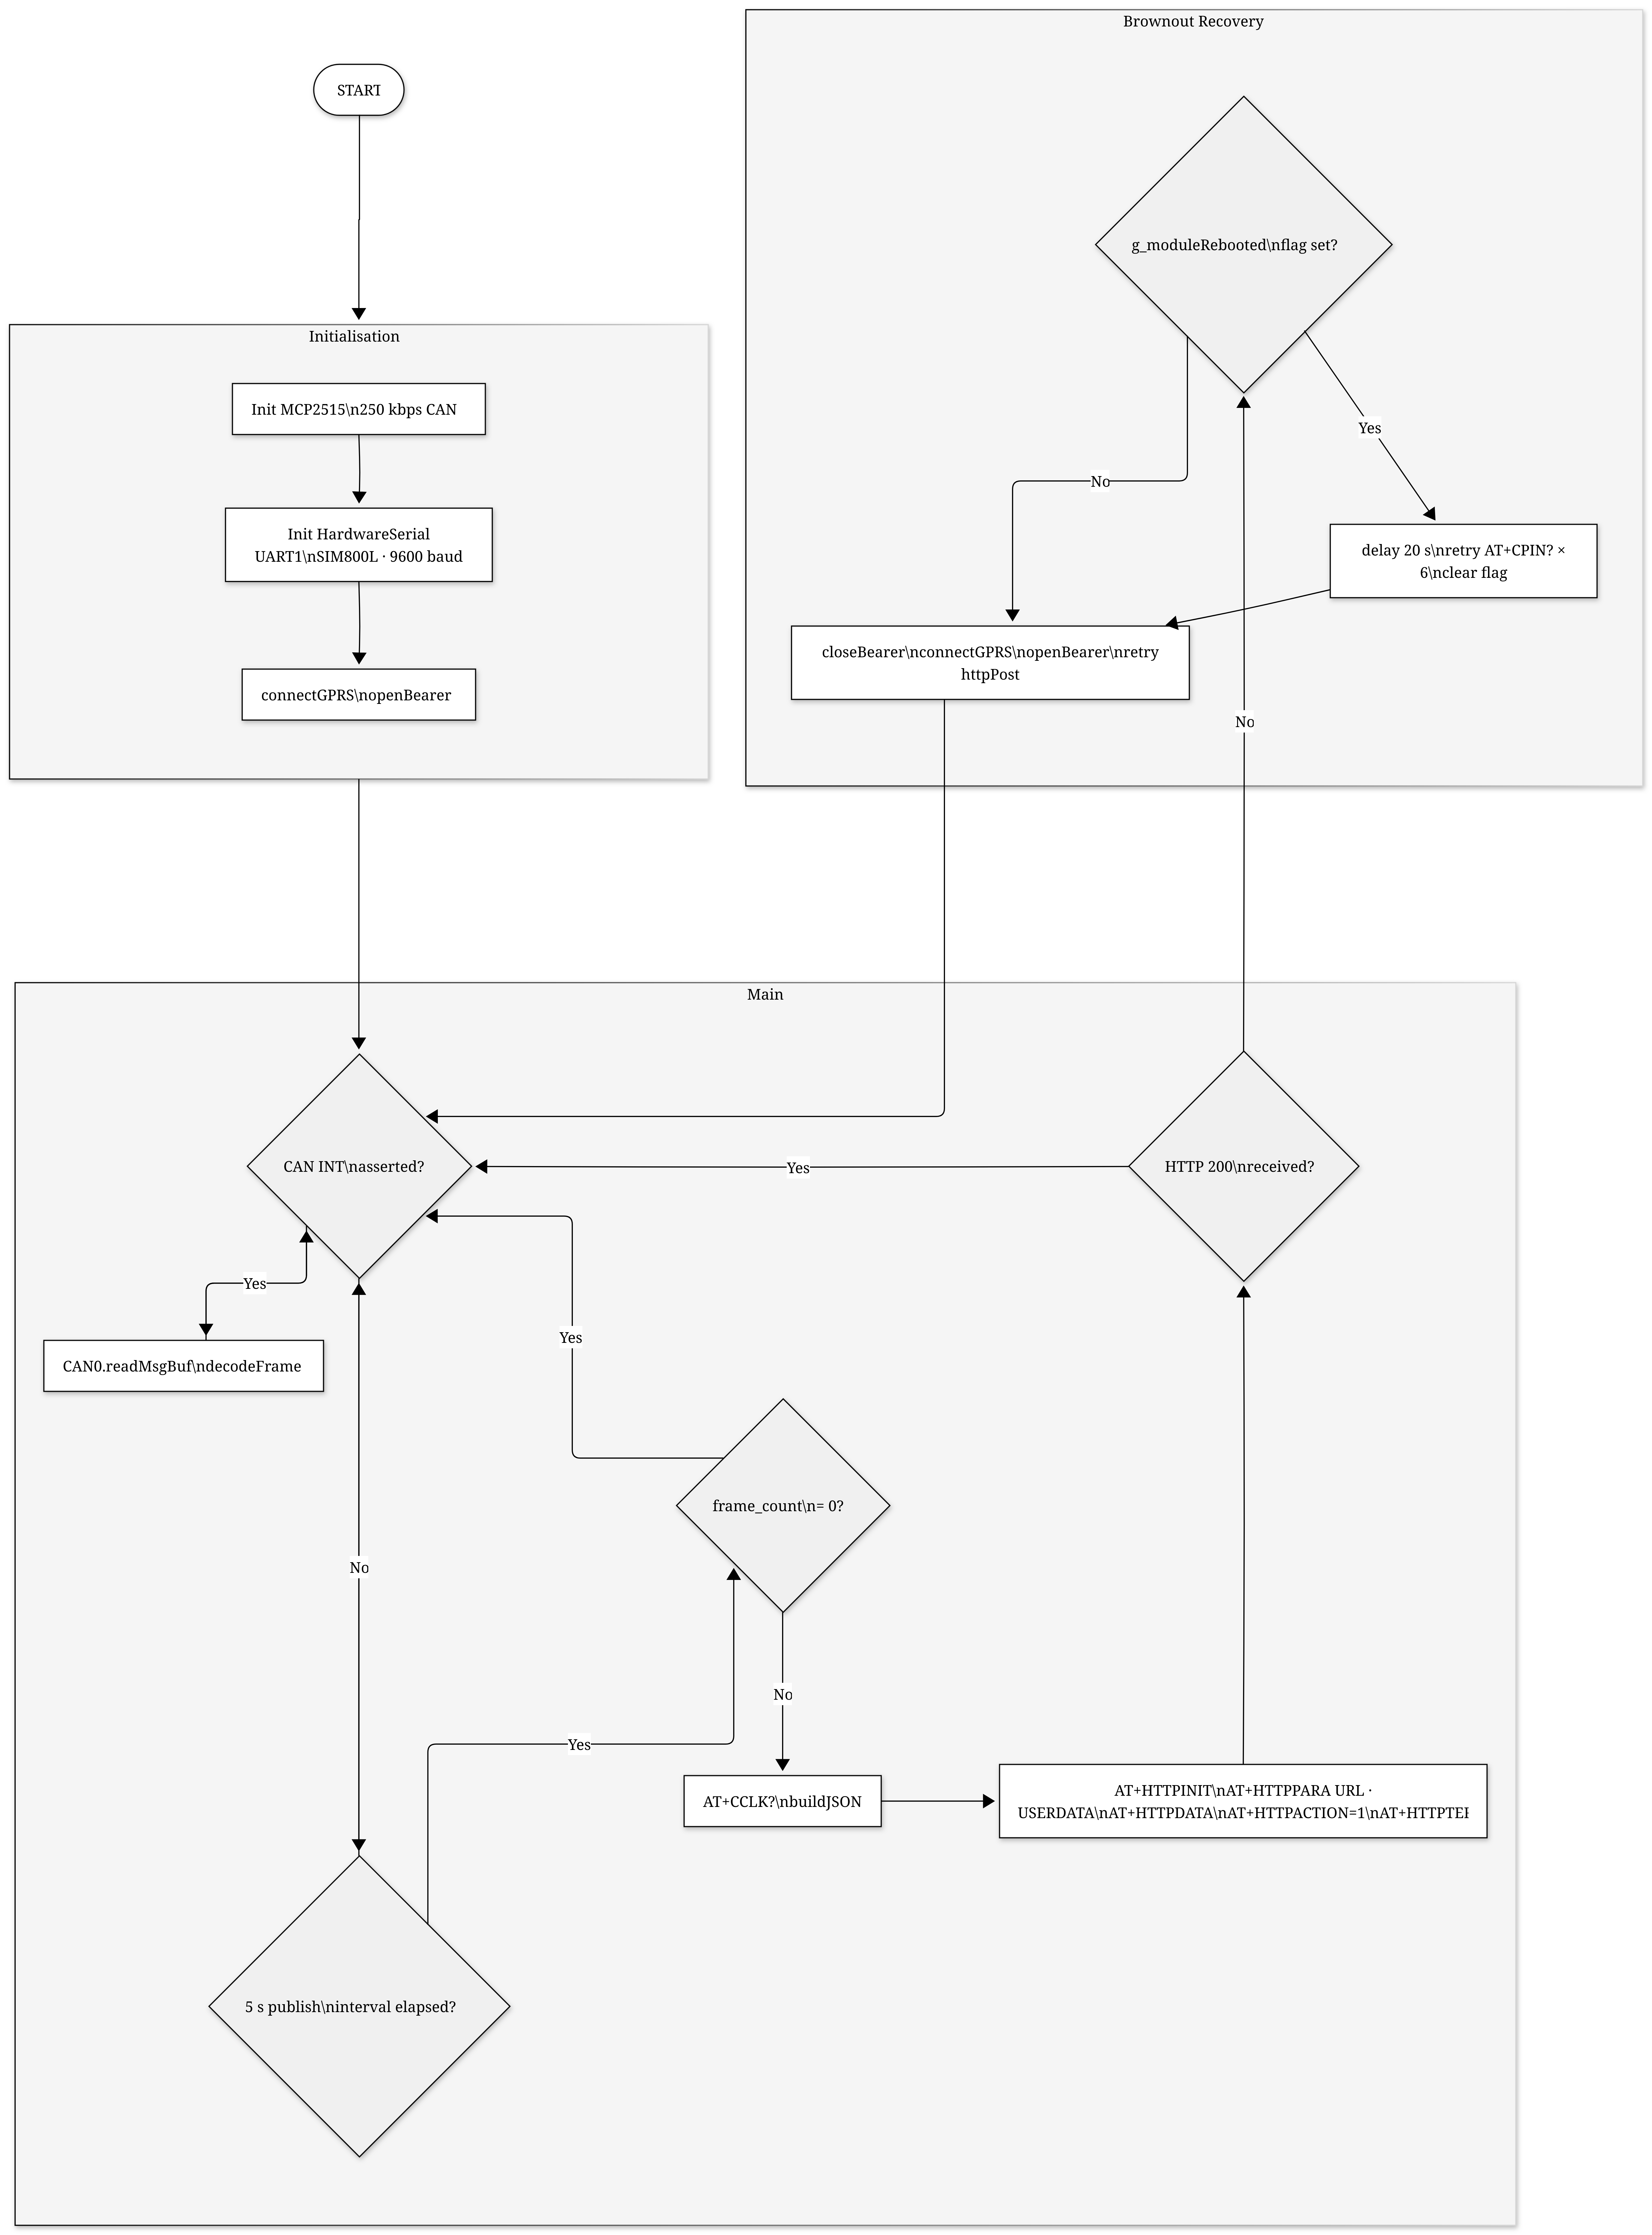
\includegraphics[width=0.7\textwidth]{images/firmware-flow-s.png}
    \caption{Firmware main-loop execution model: CAN drain $\rightarrow$ publish every 5 s}
    \label{fig:fw-flow}
\end{figure}

The SIM800L GSM modem is driven via \textbf{HardwareSerial UART1} (GPIO 16/17) at 9600 baud. HardwareSerial was chosen over SoftwareSerial because the SIM800L's AT+HTTP* responses can arrive as multi-line bursts that SoftwareSerial's byte-at-a-time interrupt handler occasionally corrupts at 9600 baud on a loaded CPU.

% ─────────────────────────────────────────────────────────────────────────────
\subsection{BMS Firmware}
\label{sec:bms-firmware}

The BMS firmware is responsible for reading raw CAN frames from the O'CELL IFS60.8-500-F-E3 battery management system, decoding them according to the \textbf{SAE J1939} standard, maintaining a live BMS state structure, and serializing that state to JSON for cloud upload.

\subsubsection{CAN Bus Interface}

The physical CAN interface uses a \textbf{MCP2515} controller connected to the ESP32 via the VSPI bus at 10 MHz. The bus operates at \textbf{250 kbps}, which is the standard J1939 baud rate for vehicle control networks. All frames from the O'CELL BMS use 29-bit extended CAN identifiers, formatted according to the J1939 Parameter Group Number (PGN) convention:

\begin{equation}
    \label{eq:j1939-id}
    \text{CAN ID} = 0x18\_\text{FUNC}\_\text{SUB}\_\text{SA}
\end{equation}

where \texttt{FUNC} is the PGN function byte that identifies the frame type, \texttt{SUB} encodes sub-addressing or destination, and \texttt{SA} = 0xF4 is the source address of the BMS module.

The MCP2515 library is configured in \texttt{MCP\_ANY} mask mode so that all frames on the bus are received without hardware filtering. Software-side filtering is performed in the \texttt{decodeFrame()} function by inspecting the \texttt{FUNC} and \texttt{SUB} bytes extracted from the 29-bit ID.

\subsubsection{Supported Frame Types}

Five distinct frame types are decoded, covering all BMS data needed for monitoring and fault diagnosis. Table~\ref{tab:can-frames} lists each frame with its CAN ID, transmission rate, and data content.

\begin{table}[h]
    \centering
    \caption{O'CELL BMS CAN Frame Map (SAE J1939, 250 kbps)}
    \label{tab:can-frames}
    \begin{tabular}{llcl}
        \toprule
        \textbf{CAN ID} & \textbf{Name} & \textbf{Rate (ms)} & \textbf{Content} \\
        \midrule
        \texttt{0x18C8--CC28F4} & Cell voltages (5 frames) & 500 & 4 cells each, big-endian uint16, 1 mV/bit \\
        \texttt{0x18B428F4}     & Temperature probes        & 500 & Up to 8 probes, raw $-$ 40 = °C \\
        \texttt{0x18FF28F4}     & BMS Basic Message 1       & 100 & SOC, current, voltage, fault flags \\
        \texttt{0x18FE28F4}     & BMS Basic Message 2       & 100 & Min/max cell mV, discharge limit \\
        \texttt{0x18FFE5F4}     & Charging request          & 500 & Max charge V, max charge A, start signal \\
        \bottomrule
    \end{tabular}
\end{table}

\paragraph{Cell Voltage Frames (0x18C8--CC28F4).}
The 19 battery cells are transmitted across five consecutive frames. Each frame carries four cells encoded as big-endian 16-bit unsigned integers, with a resolution of 1 mV per bit. The last frame (0x18CC28F4) covers cells 17--19 and pads the unused fourth slot with 0x0000. The firmware detects and skips zero-padded slots:

\begin{verbatim}
for (int i = 0; i < 4; i++) {
    uint16_t mv = u16be(data, i * 2);
    if (mv != 0 && (base + i) < 19)
        bms.cell_mv[base + i] = mv;
}
\end{verbatim}

After each group update, aggregate statistics (minimum, maximum, average) are recomputed from all non-zero cells, and a voltage-based SOC estimate is derived as described in Section~\ref{sec:soc-cal}.

\paragraph{BMS Basic Message 1 (0x18FF28F4).}
This 100 ms frame carries the core operational state of the pack. The byte layout is as follows:

\begin{itemize}
    \item \textbf{Byte 0} — Status bit-field: charge cable connected (bit 0), charging in progress (bit 1), discharging in progress (bit 2), BMS ready (bit 3), discharge contactor closed (bit 4), charge contactor closed (bit 5).
    \item \textbf{Byte 1} — State of charge from the BMS coulomb counter (0--100\%).
    \item \textbf{Bytes 2--3} — Pack current as a little-endian uint16 with a $-$5000 offset and 0.1 A/bit scaling. Positive values indicate discharge; negative values indicate charging.
    \item \textbf{Bytes 4--5} — Direct BMS pack voltage, little-endian uint16, 0.1 V/bit.
    \item \textbf{Byte 6} — Fault severity level (0 = normal, 1 = serious fault).
    \item \textbf{Byte 7} — Fault code (see Table~\ref{tab:fault-codes}).
\end{itemize}

\begin{table}[h]
    \centering
    \caption{BMS Fault Code Map (byte 7 of 0x18FF28F4)}
    \label{tab:fault-codes}
    \begin{tabular}{cl}
        \toprule
        \textbf{Code} & \textbf{Description} \\
        \midrule
        0x00 & No fault (normal operation) \\
        0x01 & Over-temperature — severe \\
        0x02 & Total pack voltage too high \\
        0x03 & Total pack voltage too low \\
        0x04 & Discharge over-current \\
        0x05 & Cell voltage too high \\
        0x06 & Cell voltage too low \\
        \bottomrule
    \end{tabular}
\end{table}

\paragraph{Temperature Probes (0x18B428F4).}
Up to eight thermal probes are encoded as single bytes using the formula $T[\text{°C}] = \text{raw} - 40$. A raw value of 0xFF indicates a disconnected sensor and is skipped. The O'CELL pack fitted to the vehicle contains four active probes.

\paragraph{Charging Request (0x18FFE5F4).}
This frame is transmitted by the BMS toward the on-board charger. It specifies the maximum allowable terminal voltage (bytes 0--1, 0.1 V/bit) and maximum charge current (bytes 2--3, 0.1 A/bit). Bit 0 of byte 4 being clear signals that the BMS is requesting the charger to begin charging.

\subsubsection{BMS State Structure}

All decoded values are accumulated into a single \texttt{BMSData} struct that persists across frames and represents the most recent complete snapshot of the battery's state. The struct is updated in-place by \texttt{decodeFrame()} and read atomically by \texttt{buildJSON()} at each publish cycle. Because the firmware runs single-threaded, no locking is required.

\subsubsection{SOC Calibration}
\label{sec:soc-cal}

The firmware uses a \textbf{voltage-based SOC estimate} derived from the average cell voltage. This method was selected because it correlates closely with the vehicle's own dashboard reading, unlike the BMS internal coulomb counter which can drift over time.

The calibration was performed over four separate on-vehicle sessions, comparing the computed average cell voltage with the vehicle's onboard display:

\begin{equation}
    \label{eq:soc}
    \text{SOC} [\%] = \frac{\overline{V}_{\text{cell}} - 2500}{3387 - 2500} \times 100
\end{equation}

where $\overline{V}_{\text{cell}}$ is the average cell voltage in millivolts. The lower bound of 2500 mV/cell corresponds to 0\% SOC (47.50 V pack), and 3387 mV/cell was calibrated to match 100\% on the car display (64.35 V pack). Values above 3387 mV, which occur during active charging, are clamped to 100\%.

Table~\ref{tab:soc-cal} shows the four calibration sessions used to arrive at the 3387 mV reference point.

\begin{table}[h]
    \centering
    \caption{SOC Calibration Data — Four On-Vehicle Sessions}
    \label{tab:soc-cal}
    \begin{tabular}{cccc}
        \toprule
        \textbf{Session} & \textbf{Avg cell (mV)} & \textbf{Car display (\%)} & \textbf{Solved top (mV)} \\
        \midrule
        2026-03-31 10:06 & 3301.6 & 89.0 & 3400.7 \\
        2026-03-31 10:57 & 3306.2 & 89.0 & 3405.8 \\
        2026-04-01 13:03 & 3284.8 & 89.4 & 3377.9 \\
        2026-04-01 16:04 & 3285.0 & 88.4 & 3387.4 \\
        \midrule
        \multicolumn{3}{r}{\textbf{Adopted reference}} & \textbf{3387 mV} \\
        \bottomrule
    \end{tabular}
\end{table}

\subsubsection{Cloud Publishing via SIM800L}

At every 5-second publish interval, the firmware calls \texttt{buildJSON()} to serialize the current \texttt{BMSData} struct into a JSON string, then calls \texttt{httpPost()} to deliver it to the VPS backend via SIM800L GPRS.

The HTTP transaction uses the SIM800L's native \textbf{AT+HTTP*} command set over plain HTTP (AT+HTTPSSL=0). The sequence is:

\begin{enumerate}
    \item \texttt{AT+HTTPTERM} — close any stale session from a previous transaction.
    \item \texttt{AT+HTTPINIT} — open a new HTTP session.
    \item \texttt{AT+HTTPPARA="URL",...} — set the full endpoint URL.
    \item \texttt{AT+HTTPPARA="USERDATA","X-Api-Key: \textit{key}\textbackslash r\textbackslash n"} — inject the API authentication header.
    \item \texttt{AT+HTTPDATA=\textit{len},10000} — upload the JSON body.
    \item \texttt{AT+HTTPACTION=1} — execute the HTTP POST and wait for \texttt{+HTTPACTION:} response.
    \item \texttt{AT+HTTPTERM} — close the session.
\end{enumerate}

During the AT+HTTPACTION wait loop (up to 30 s), the firmware continues draining CAN frames from the MCP2515 receive buffer so that no BMS data is lost while the modem is busy.

\subsubsection{Brownout Recovery}

A known failure mode of the SIM800L is a mid-transaction power brownout caused by the $\sim$1.5 A peak current during GPRS transmission exceeding the supply rail's transient capability. When this occurs, the modem resets and emits an unsolicited \texttt{"Call Ready"} string in its UART output.

The firmware detects this string in every AT response buffer (both \texttt{sendAT()} and \texttt{sendATExpect()} and the \texttt{HTTPACTION} wait loop) and sets a global \texttt{g\_moduleRebooted} flag. When a publish cycle fails and this flag is set, the recovery sequence is:

\begin{enumerate}
    \item Wait 20 s for the SIM card and GSM stack to re-initialize.
    \item Retry \texttt{AT+CPIN?} up to six times at 4-second intervals.
    \item Re-open the GPRS bearer and retry the publish once more.
\end{enumerate}

The long-term hardware fix is to add a 1000 µF / 10 V bulk capacitor close to the SIM800L VCC pin.

% ─────────────────────────────────────────────────────────────────────────────
\subsection{Motor Control Algorithms}
% Content placeholder — to be completed by the Motor Control team

% ─────────────────────────────────────────────────────────────────────────────
\subsection{Vehicle Management Unit (VMU) Software}
% Content placeholder — to be completed by the VMU team

% ─────────────────────────────────────────────────────────────────────────────
\subsection{OTA Update \& Secure Boot}
% Content placeholder — to be completed by the embedded systems team

% ─────────────────────────────────────────────────────────────────────────────
\subsection{Unit \& Integration Testing}

Software testing for the BMS firmware and cloud pipeline was conducted at three levels: unit testing of the decoding logic, integration testing of the full CAN-to-cloud pipeline, and functional testing of the live dashboard.

\subsubsection{Unit Testing — Frame Decoder}

Each frame type in \texttt{decodeFrame()} was verified by replaying known raw bytes and checking the decoded output against hand-computed expected values. The test case below illustrates verification of cell voltage frame 0x18CB28F4:

\begin{verbatim}
Frame ID: 0x18CB28F4   Data: 0D 3F  0D 38  0D 3A  0D 39

0x0D3F = 3391 mV  -> Cell 13   (big-endian, group = 0xCB - 0xC8 = 3)
0x0D38 = 3384 mV  -> Cell 14
0x0D3A = 3386 mV  -> Cell 15
0x0D39 = 3385 mV  -> Cell 16
\end{verbatim}

Similarly, the signed current decoding formula (offset $-$5000, scale 0.1 A/bit) and the SOC formula (Equation~\eqref{eq:soc}) were verified against values from the real car log file \texttt{bms\_log\_2026-03-10T10-20-02.txt}, which contains 3197 frames captured during an on-vehicle session.

\subsubsection{Integration Testing — Cloud Pipeline}

The end-to-end pipeline was tested without live hardware using the \texttt{replay\_to\_cloud.py} tool, which parses the captured CAN log and replays decoded JSON snapshots to \texttt{POST /api/ingest} at configurable speed. This allowed the following verifications:

\begin{itemize}
    \item The \texttt{/api/ingest} endpoint correctly rejects requests with an invalid \texttt{X-Api-Key} header (HTTP 401).
    \item Each accepted snapshot is stored in the SQLite \texttt{bms\_cloud.db} database with correct timestamp and device ID.
    \item The \texttt{/ws/cloud} WebSocket pushes the most recent snapshot to all connected browser clients within 2 seconds of ingestion.
    \item The \texttt{/api/history} endpoint returns records newest-first with correct JSON structure.
\end{itemize}

\subsubsection{Functional Testing — Live Dashboard}

The live dashboard (\texttt{frontend/index.html}) was tested in both SERIAL and CLOUD modes:

\begin{description}
    \item[SERIAL mode] ESP32 connected via USB to a development laptop. The server decoded incoming frames in real time and the 19-cell voltage grid, SOC ring, and temperature bars updated at 10 Hz without visible lag.
    \item[CLOUD mode] Data replayed from the log file through \texttt{/api/ingest}. The dashboard received snapshots via \texttt{/ws/cloud} at 2 Hz and all panels rendered correctly, including the cloud communication log panel which displayed timestamped RECV and WS events.
    \item[Reconnect behavior] The backend was deliberately stopped while the dashboard was open. The browser WebSocket closed, the connection status indicator turned red (Disconnected), and the overlay appeared. On server restart, the client automatically reconnected within 5 seconds and resumed live updates.
\end{description}
